%!TEX root = ../thesis.tex
%*******************************************************************************
%****************************** Third Chapter **********************************
%*******************************************************************************
\chapter{Conclusiones y trabajo futuro}\label{chap:concl}

\begin{graybox}
\begin{itemize}
\item La extensión \pgland{} simplifica algunas complejas consultas SQL que son necesarias para calcular métricas del paisaje en una geodatabase.
\item El rendimiento de las consultas resulta prometedor, lo que permitirá crear servicios web de consulta directa sobre el SIOSE y bases de datos similares.   
\item El trabajo con \textit{dockers} facilita la reproducibilidad de la investigación y un despliegue escalable en Internet.
\item Los conocimientos adquiridos en el Máster sirven como introducción campos profesionales muy amplios.
\end{itemize}
\end{graybox}

Los objetivos planteados en el capítulo de \nameref{chap:intro} comprendian aspectos de trabajo colaborativo, cuestiones tecnológicas y había una gran preocupación por mejorar la \textit{usabilidad} de bases de datos voluminosas y complejas como la del SIOSE. En este sentido, el objetivo principal se ha conseguido al contribuir significativamente en el \textbf{desarrollo de una extensión de Postgres/PostGIS que facilita en gran medida el cálculo de métricas del paisaje}. 

La encapsulación del cálculo de métricas del paisaje en funciones de PostgreSQL/PostGIS facilita en gran medida la realización de estos cálculos a partir de bases de datos de ocupación del suelo como la del SIOSE. Esta facilidad se evidencia en la \textbf{reducción del número de líneas de SQL necesarias para el cálculo de las distintas métricas del paisaje}. Además, el desarrollo de nuevas métricas se ha podido sistematizar gracias a la gran extensibilidad de PostgreSQL/PostGIS. El uso de las más recientes tecnologías (\textit{Git y Dockers}) permite repartir el trabajo de desarrollo en equipos multidisciplinares, como lo es el del Laboratorio de Geomática de la Universidad de Alicante.

En este trabajo se ha obtenido un prototipo de una aplicación que, según los objetivos del Proyecto SIOSE-INNOVA, se pretende desarrollar en unos tres años. El desarrollo de una extensión \textit{en producción} llevará más tiempo, es un trabajo complejo que requiere de todo un equipo de expertos y meses de trabajo, es por ello que \textbf{el trabajo en equipo es esencial en este tipo de proyectos.}

\begin{figure}
\begin{center}
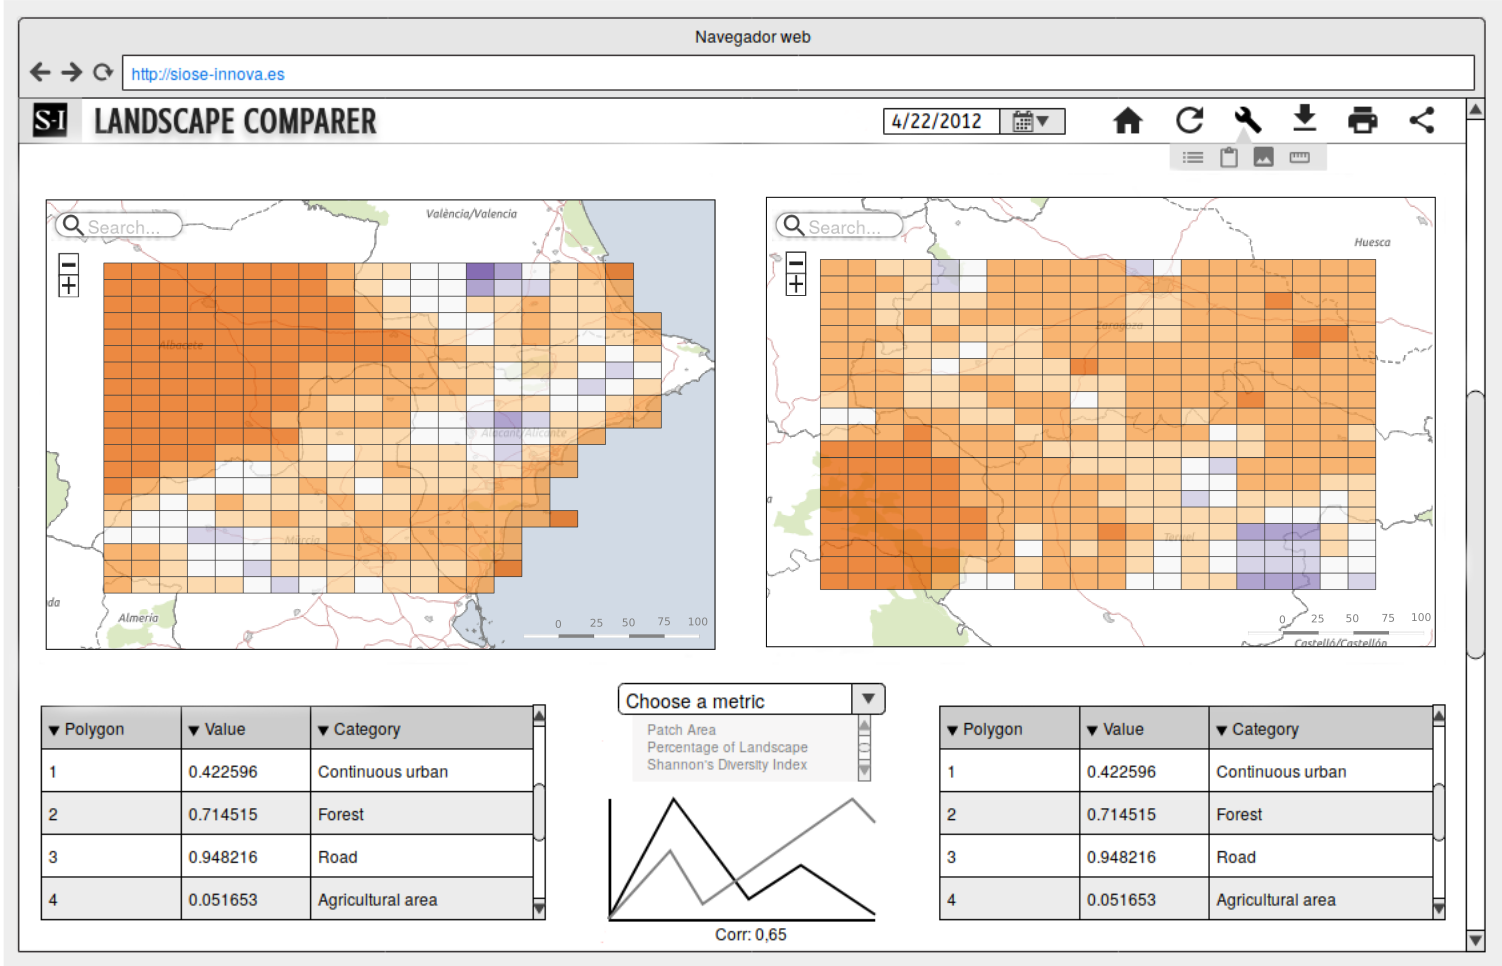
\includegraphics[width=\textwidth]{ConclusionyFuturo/Figs/visor-final.png}
\caption{Ejemplo de comparación de estructuras de paisaje a partir del SIOSE mediante el visor cartográfico . \label{fig:visor-final}}
\end{center}
\end{figure}

Los resultados obtenidos en el caso de uso descrito en las secciones \ref{sec:exp} y \ref{sec:caso_uso} han servido para poner a prueba la extensión y el resto de tecnologías en cuanto a su potencial de aplicación. Directamente sobre la geodatabase del SIOSE, se ha comprobado que es posible realizar centenares de consultas sobre métricas del paisaje en unos pocos segundos, y todo ello en un ordenador de sobremesa. Más aún, las nuevas tecnologías de contenerización utilizadas (\textit{Dockers}) permiten desplegar y distribuir toda la plataforma descrita en este trabajo en uno o varios servidores de Internet, por lo que cabe pensar que este tipo de servicios podrían ser ofrecidos a un gran número de usuarios del SIOSE.

Tras redactar este trabajo es posible valorar aún más los contenidos del ``Máster en Tecnologías de la Información Geográfica para la Ordenación del Territorio: SIG y Teledetección''. En las asignaturas de \textit{fundamentos teóricos sobre bases de datos, diseño e implementación de bases de datos, lenguajes de programación, software libre, análisis espacial básico, análisis visual de imágenes y desarrollo e implementación de la información geográfica en aplicaciones infográficas} se adquirieron conocimientos básicos para empezar a trabajar en un proyecto avanzado sobre geodatabases, como el propuesto en el marco del proyecto SIOSE-INNOVA.
